\documentclass[svgnames,11pt]{beamer}
\setbeamercolor{structure}{fg=SlateGray}
\usetheme{Goettingen}
\input{/home/tof/Documents/Cozy/latex-include/preambule_commun.tex}
\usepackage{pgfpages}
\setbeameroption{show notes on second screen=left}
\author[]{Christophe Viroulaud}
\title{Architecture d'un système informatique embarqué}
\date{}
%\logo{}
\institute{Seconde SNT}
%\institute{Première NSI}
%\institute{Terminale NSI}
\setbeamertemplate{navigation symbols}{}
\setbeamertemplate{footline}[frame number]
\setbeamertemplate{section in toc}[sections numbered]
\setbeamertemplate{subsection in toc}[subsections numbered]

\newif\iflattersubsect
\AtBeginSection{
    \begin{frame}{Sommaire}
        \tableofcontents[sectionstyle=show/shaded,subsectionstyle=show/shaded/hide ]
        \end{frame} 
        \lattersubsectfalse
}
\AtBeginSubsection[]{
    \iflattersubsect
    \begin{frame}{Sommaire}
        \tableofcontents[sectionstyle=show/shaded,subsectionstyle=show/shaded/hide ]
      \end{frame} 
      \fi
    \lattersubsecttrue
}

\begin{document}
\begin{frame}
    \titlepage
\end{frame}

\section{Problématique}
\begin{frame}
    \frametitle{Problématique}

    Les ordinateurs sont de plus en plus présents dans les objets qui nous entourent. Mais même si le principe reste équivalent, il y a des différences entre un ordinateur de bureau et un système embarqué.

\end{frame}
\begin{frame}
    \frametitle{}

    \begin{center}
        \centering
        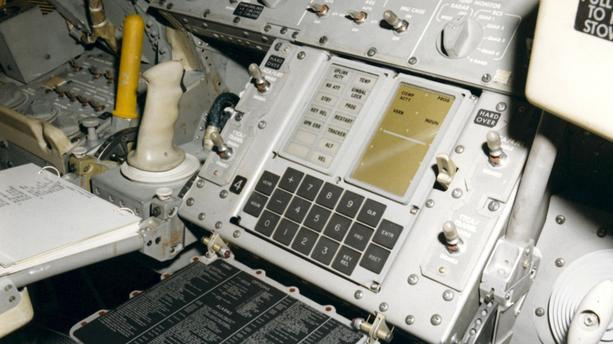
\includegraphics[width=8cm]{ressources/apollo.jpeg}
        \captionof{figure}{\textbf{1967: }premier système embarqué de guidage lors de la mission lunaire Apollo}
        \label{IMG}
    \end{center}

\end{frame}
\begin{frame}
    \frametitle{}

    \begin{center}
        \centering
        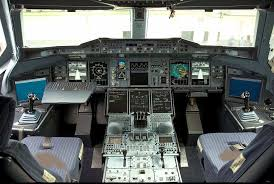
\includegraphics[width=8cm]{ressources/a320.jpeg}
        \captionof{figure}{\textbf{1984: }Airbus 320, premier avion équipé de commandes électriques informatisées}
        \label{IMG}
    \end{center}

\end{frame}
\begin{frame}
    \frametitle{}

    \begin{center}
        \centering
        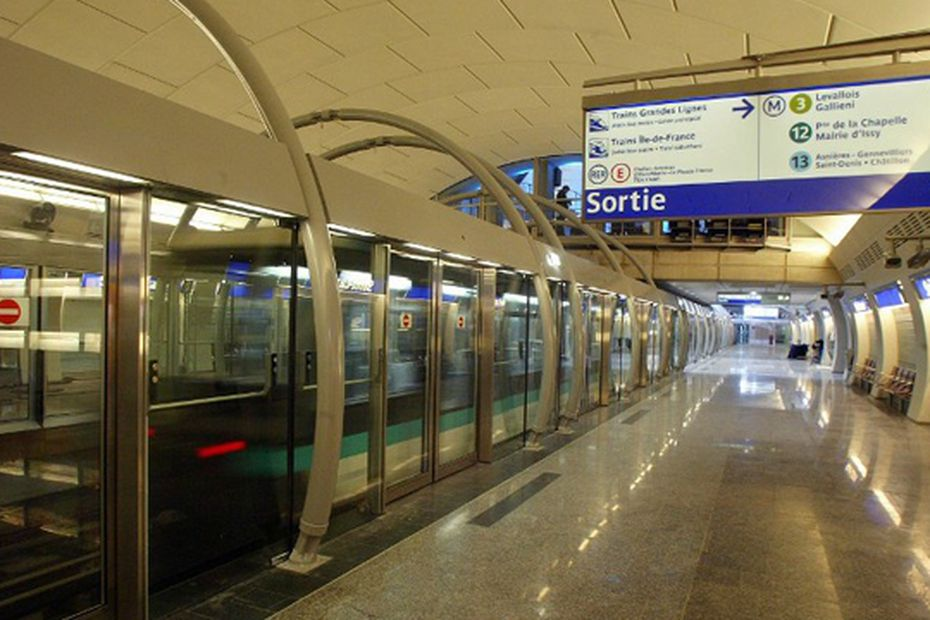
\includegraphics[width=8cm]{ressources/metro.jpg}
        \captionof{figure}{\textbf{1998: }métro informatisé sans conducteur Météor (ligne 14 à Paris)}
        \label{IMG}
    \end{center}

\end{frame}
\begin{frame}
    \frametitle{}

    \begin{center}
        \centering
        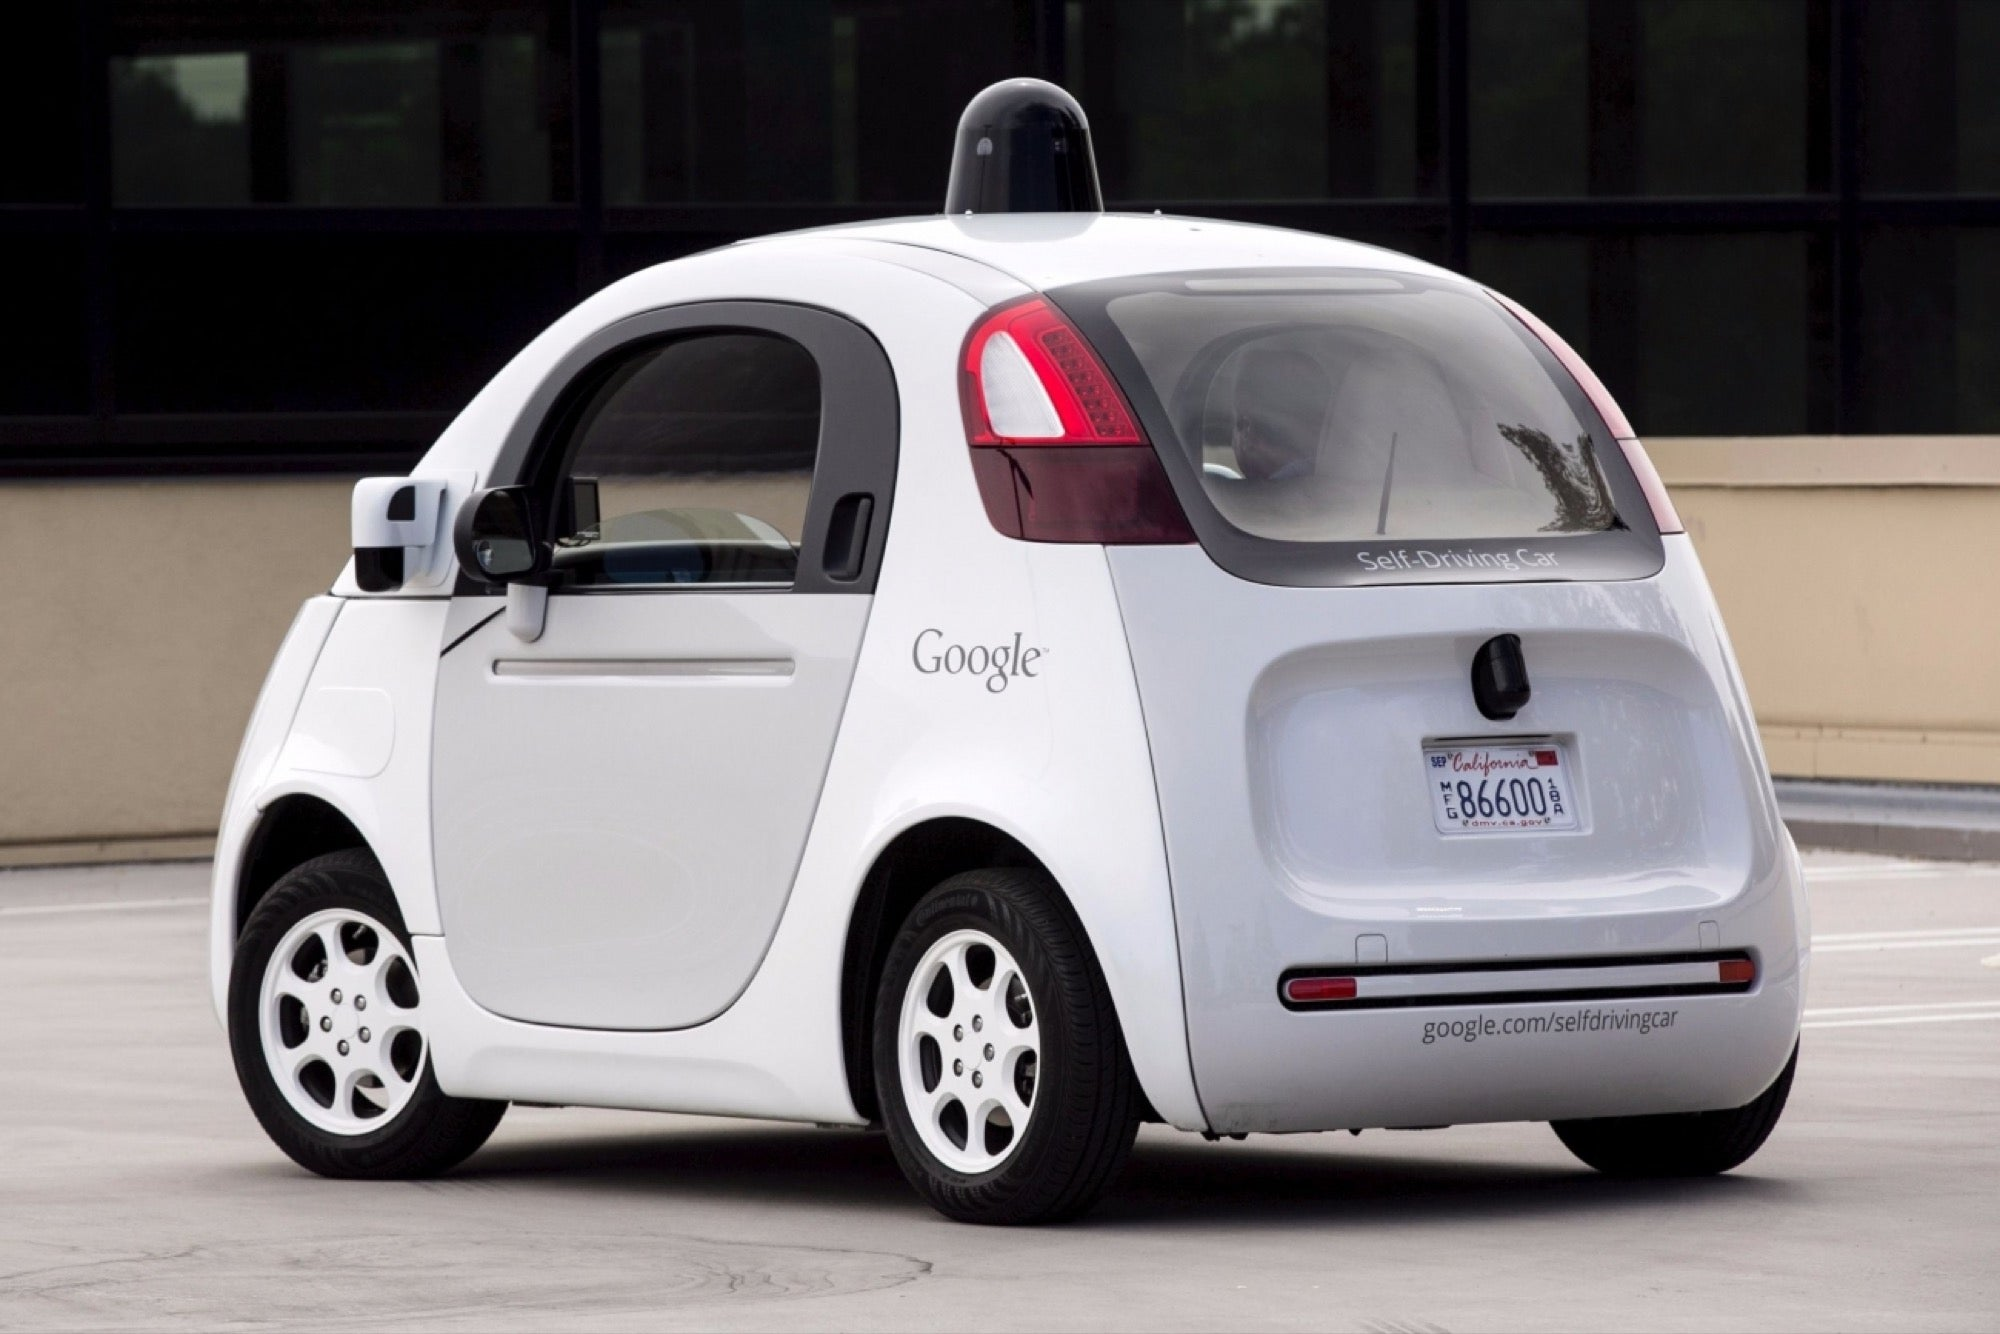
\includegraphics[width=8cm]{ressources/voiture.jpg}
        \captionof{figure}{\textbf{2009: }le projet Auto-Driving Car de Google a débuté}
        \label{IMG}
    \end{center}

\end{frame}
\begin{frame}
    \frametitle{}
    \begin{center}
        \framebox{Comment embarquer un ordinateur dans un objet?}
    \end{center}


\end{frame}

\section{Architecture d'un ordinateur embarqué}
\subsection{Principe général d'un ordinateur}
\begin{frame}
    \frametitle{Principe général d'un ordinateur}

    Un système embarqué est avant tout un ordinateur. Il est composé:
    \begin{itemize}
        \item<1-> d'un \emph{processeur} qui exécute les instructions d'un programme,
        \item<2-> d'une \emph{mémoire} qui stocke les programmes et les données.
    \end{itemize}

\end{frame}
\begin{frame}
    \frametitle{}

    Pour communiquer avec un ordinateur on utilise des \emph{interfaces homme-machine (IHM)}:
    \begin{itemize}
        \item<1-> les \emph{périphériques d'entrée} pour lui donner des informations,
        \item<2-> les \emph{périphériques de sortie} pour visualiser le résultat des programmes exécutés.
    \end{itemize}

\end{frame}
\begin{frame}
    \frametitle{}
    \begin{activite}
        Citer différents périphériques d'entrée et sortie.
    \end{activite}


\end{frame}
\begin{frame}
    \frametitle{Correction}
    \begin{itemize}
        \item \emph{Périphériques d'entrée:} clavier, souris, joystick, micro, webcam\dots
        \item \emph{Périphériques de sortie: }écran, haut-parleur, imprimante\dots
    \end{itemize}


\end{frame}
\subsection{Interagir avec le monde extérieur}
\begin{frame}
    \frametitle{Interagir avec le monde extérieur}

    Dans une voiture autonome Google il n'y a ni volant ni pédale. Pour interagir avec le monde extérieur, la voiture utilise:
    \begin{itemize}
        \item<1-> des \emph{capteurs} pour obtenir des informations du monde réel et les envoyer sous forme numérique à l'ordinateur,
        \item<2-> des \emph{actionneurs} pour modifier le comportement de la voiture en fonction des instructions de l'ordinateur.
    \end{itemize}

\end{frame}
\begin{frame}
    \frametitle{}

    \begin{center}
        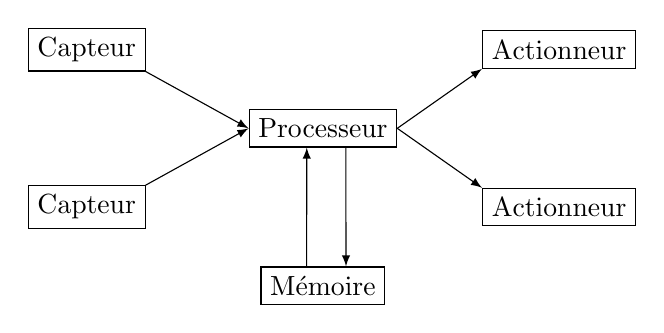
\begin{tikzpicture}
            \node[draw] (p)at(0,0) {Processeur};
            \node[draw] (m)at(0,-2) {Mémoire};
            \node[draw] (c1)at(-3,1) {Capteur};
            \node[draw] (c2)at(-3,-1) {Capteur};
            \node[draw] (a1)at(3,1) {Actionneur};
            \node[draw] (a2)at(3,-1) {Actionneur};
            \draw[->,>=latex] (p.-40) -- (m.40);
            \draw[->,>=latex] (m.130) -- (p.-130);
            \draw[->,>=latex] (c1.south east) -- (p.west);
            \draw[->,>=latex] (c2.north east) -- (p.west);
            \draw[->,>=latex] (p.east) -- (a1.south west);
            \draw[->,>=latex] (p.east) -- (a2.north west);

        \end{tikzpicture}
        \captionof{figure}{Système embarqué}
        \label{sie}
    \end{center}

\end{frame}
\begin{frame}
    \frametitle{}

    \begin{activite}
        \begin{enumerate}
            \item Dans un système embarqué qu'est-ce qui remplace les périphériques d'entrée?
            \item Établir un schéma du système embarqué d'une voiture autonome.
        \end{enumerate}
    \end{activite}

\end{frame}
\begin{frame}
    \frametitle{Correction}

    Dans un système embarqué les \emph{capteurs} remplacent les périphériques d'entrée.

\end{frame}
\begin{frame}
    \frametitle{Correction}

    \begin{center}
        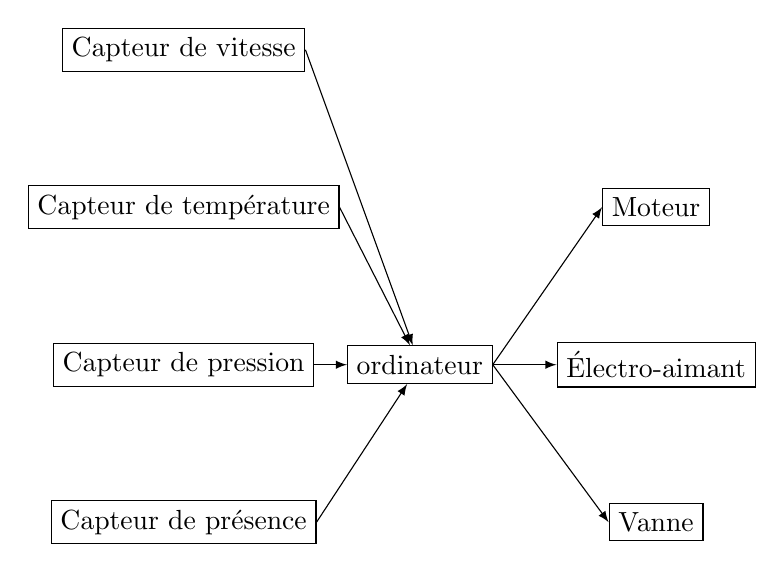
\begin{tikzpicture}
            \node[draw] (p)at(0,0) {ordinateur};
            \node[draw] (c1)at(-3,4) {Capteur de vitesse};
            \node[draw] (c2)at(-3,2) {Capteur de température};
            \node[draw] (c3)at(-3,0) {Capteur de pression};
            \node[draw] (c4)at(-3,-2) {Capteur de présence};

            \node[draw] (a1)at(3,2) {Moteur};
            \node[draw] (a2)at(3,0) {Électro-aimant};
            \node[draw] (a3)at(3,-2) {Vanne};

            \draw[->,>=latex] (c1.east) -- (p);
            \draw[->,>=latex] (c2.east) -- (p);
            \draw[->,>=latex] (c3.east) -- (p);
            \draw[->,>=latex] (c4.east) -- (p);

            \draw[->,>=latex] (p.east) -- (a1.west);
            \draw[->,>=latex] (p.east) -- (a2.west);
            \draw[->,>=latex] (p.east) -- (a3.west);

        \end{tikzpicture}
        \captionof{figure}{Voiture autonome}
        \label{sie}
    \end{center}
    \note[item]{vanne: ouvre ferme arrivée essence}
    \note[item]{pression: pneu}
    \note[item]{humidité: essuie-glace}
    \note[item]{électro-aimant: moteurs électriques (essuie-glace) $\rightarrow$ produit aimantation grâce courant électrique}
    \note[item]{accéléromètre, lumière}
\end{frame}
\end{document}